%Copyright  Jean-Philippe Eisenbarth
%This program is free software: you can 
%redistribute it and/or modify it under the terms of the GNU General Public 
%License as published by the Free Software Foundation, either version 3 of the 
%License, or (at your option) any later version.
%This program is distributed in the hope that it will be useful,but WITHOUT ANY 
%WARRANTY; without even the implied warranty of MERCHANTABILITY or FITNESS FOR A 
%PARTICULAR PURPOSE. See the GNU General Public License for more details.
%You should have received a copy of the GNU General Public License along with 
%this program.  If not, see <http://www.gnu.org/licenses/>.

%Based on the code of Yiannis Lazarides
%http://tex.stackexchange.com/questions/42602/software-requirements-specification-with-latex
%http://tex.stackexchange.com/users/963/yiannis-lazarides
%Also based on the template of Karl E. Wiegers
%http://www.se.rit.edu/~emad/teaching/slides/srs_template_sep14.pdf
%http://karlwiegers.com
\documentclass{scrreprt}
\usepackage{array}
\usepackage{listings}
\usepackage{underscore}
\usepackage[bookmarks=true]{hyperref}
\usepackage[utf8]{inputenc} 
\usepackage[english]{babel}
\usepackage{textcomp}
\usepackage{graphicx} %utilisation d'images
\hypersetup{
    bookmarks=false,    % show bookmarks bar?
    pdftitle={Software Requirement Specification},    % title
    pdfauthor={Jean-Philippe Eisenbarth},                     % author
    pdfsubject={TeX and LaTeX},                        % subject of the document
    pdfkeywords={TeX, LaTeX, graphics, images}, % list of keywords
    colorlinks=true,       % false: boxed links; true: colored links
    linkcolor=blue,       % color of internal links
    citecolor=black,       % color of links to bibliography
    filecolor=black,        % color of file links
    urlcolor=purple,        % color of external links
    linktoc=page            % only page is linked
}%
\def\myversion{1.0 }
\date{}
%\title
\usepackage{hyperref}
\begin{document}

\begin{flushright}
    \rule{15cm}{5pt}\vskip1cm
    \begin{bfseries}
        \Huge{SOFTWARE REQUIREMENTS\\ SPECIFICATION}\\
        \vspace{1.0cm}
        for\\
        \vspace{1.0cm}
        Gestionnaire de Stage Telecom Nancy\\
        \vspace{1.0cm}
        \LARGE{version \myversion approved}\\
        
        \vspace{1.0cm}
        Prepared by \\ 
        \vspace{1.0cm}
        \begin{flushleft}
        Alexandre Chichmanian \\ Gauthier Zambaux \\ Mouchid Waidi \\ Guillaume Garcia\\
        \end{flushleft}
        \vspace{1.0cm}
        Los Pollos\\
        \vspace{1.0cm}
        \today\\
    \end{bfseries}
\end{flushright}

\renewcommand{\contentsname}{Contenu}
\tableofcontents


\chapter*{Revision History}

\begin{center}
    \begin{tabular}{|c|c|c|c|}
        \hline
	    Name & Date & Reason For Changes & Version\\
        \hline
	    21 & 22 & 23 & 24\\
        \hline
	    31 & 32 & 33 & 34\\
        \hline
    \end{tabular}
\end{center}

\chapter{INTRODUCTION}

\section{A propos de ce document}
$<$Identify the product whose software requirements are specified in this 
document, including the revision or release number. Describe the scope of the 
product that is covered by this SRS, particularly if this SRS describes only 
part of the system or a single subsystem.$>$

\section{Portée du document}
$<$Describe any standards or typographical conventions that were followed when 
writing this SRS, such as fonts or highlighting that have special significance.  
For example, state whether priorities  for higher-level requirements are assumed 
to be inherited by detailed requirements, or whether every requirement statement 
is to have its own priority.$>$

\section{Public concerné et vue d'ensemble du document }
$<$Describe the different types of reader that the document is intended for, 
such as developers, project managers, marketing staff, users, testers, and 
documentation writers. Describe what the rest of this SRS contains and how it is 
organized. Suggest a sequence for reading the document, beginning with the 
overview sections and proceeding through the sections that are most pertinent to 
each reader type.$>$

\section{Définitions, acronymes et abréviations}
$<$Provide a short description of the software being specified and its purpose, 
including relevant benefits, objectives, and goals. Relate the software to 
corporate goals or business strategies. If a separate vision and scope document 
is available, refer to it rather than duplicating its contents here.$>$

\section{Conventions de rédaction du document}
$<$List any other documents or Web addresses to which this SRS refers. These may 
include user interface style guides, contracts, standards, system requirements 
specifications, use case documents, or a vision and scope document. Provide 
enough information so that the reader could access a copy of each reference, 
including title, author, version number, date, and source or location.$>$

\section{Références et remerciements}
$<$List any other documents or Web addresses to which this SRS refers. These may 
include user interface style guides, contracts, standards, system requirements 
specifications, use case documents, or a vision and scope document. Provide 
enough information so that the reader could access a copy of each reference, 
including title, author, version number, date, and source or location.$>$


\chapter{DESCRIPTION GLOBALE }

\section{Perspective du produit}
$<$Describe the context and origin of the product being specified in this SRS.  
For example, state whether this product is a follow-on member of a product 
family, a replacement for certain existing systems, or a new, self-contained 
product. If the SRS defines a component of a larger system, relate the 
requirements of the larger system to the functionality of this software and 
identify interfaces between the two. A simple diagram that shows the major 
components of the overall system, subsystem interconnections, and external 
interfaces can be helpful.$>$

\section{Fonctionnalités du produit}
$<$Summarize the major functions the product must perform or must let the user 
perform. Details will be provided in Section 3, so only a high level summary 
(such as a bullet list) is needed here. Organize the functions to make them 
understandable to any reader of the SRS. A picture of the major groups of 
related requirements and how they relate, such as a top level data flow diagram 
or object class diagram, is often effective.$>$

\section{Utilisateurs}
$<$Identify the various user classes that you anticipate will use this product.  
User classes may be differentiated based on frequency of use, subset of product 
functions used, technical expertise, security or privilege levels, educational 
level, or experience. Describe the pertinent characteristics of each user class.  
Certain requirements may pertain only to certain user classes. Distinguish the 
most important user classes for this product from those who are less important 
to satisfy.$>$

\section{Environnement d'exécution}
$<$Describe the environment in which the software will operate, including the 
hardware platform, operating system and versions, and any other software 
components or applications with which it must peacefully coexist.$>$

\section{Contraintes de conception et d'implémentation}
$<$Describe any items or issues that will limit the options available to the 
developers. These might include: corporate or regulatory policies; hardware 
limitations (timing requirements, memory requirements); interfaces to other 
applications; specific technologies, tools, and databases to be used; parallel 
operations; language requirements; communications protocols; security 
considerations; design conventions or programming standards (for example, if the 
customerés organization will be responsible for maintaining the delivered 
software).$>$

\section{Manuel utilisateur}
$<$List the user documentation components (such as user manuals, on-line help, 
and tutorials) that will be delivered along with the software. Identify any 
known user documentation delivery formats or standards.$>$


\section{Hypothèses et dépendances}
$<$List any assumed factors (as opposed to known facts) that could affect the 
requirements stated in the SRS. These could include third-party or commercial 
components that you plan to use, issues around the development or operating 
environment, or constraints. The project could be affected if these assumptions 
are incorrect, are not shared, or change. Also identify any dependencies the 
project has on external factors, such as software components that you intend to 
reuse from another project, unless they are already documented elsewhere (for 
example, in the vision and scope document or the project plan).$>$


\chapter{BESOINS SPÉCIFIQUES}

\section{Besoins externes}
$<$Describe the logical characteristics of each interface between the software 
product and the users. This may include sample screen images, any GUI standards 
or product family style guides that are to be followed, screen layout 
constraints, standard buttons and functions (e.g., help) that will appear on 
every screen, keyboard shortcuts, error message display standards, and so on.  
Define the software components for which a user interface is needed. Details of 
the user interface design should be documented in a separate user interface 
specification.$>$

\section{Besoins fonctionnels}
$<$Describe the logical and physical characteristics of each interface between 
the software product and the hardware components of the system. This may include 
the supported device types, the nature of the data and control interactions 
between the software and the hardware, and communication protocols to be 
used.$>$

\section{Besoins comportementaux}
$<$Describe the connections between this product and other specific software 
components (name and version), including databases, operating systems, tools, 
libraries, and integrated commercial components. Identify the data items or 
messages coming into the system and going out and describe the purpose of each.  
Describe the services needed and the nature of communications. Refer to 
documents that describe detailed application programming interface protocols.  
Identify data that will be shared across software components. If the data 
sharing mechanism must be implemented in a specific way (for example, use of a 
global data area in a multitasking operating system), specify this as an 
implementation constraint.$>$
\subsection{Diagrammes de séquence des cas d'utilisation}
%AUTENTIFICATION :
\begin{center}
	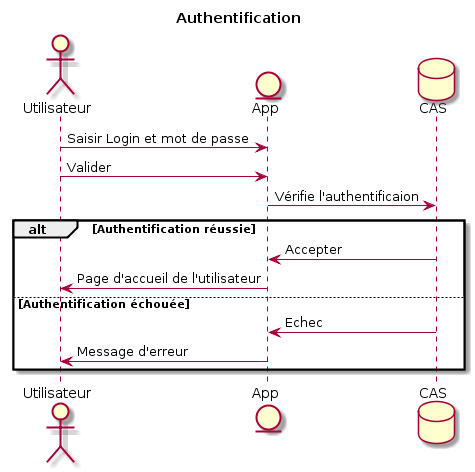
\includegraphics[scale=0.55]{image/authentification.png}
\end{center}
%\begin{center}
%	\textbf{Figure 3.3.1.} S'autentifier
%\end{center}
\hspace{1cm}Les utilisateurs de l'application doivent s'y authentifier à son ouverture. Ils utilisent pour cela leurs identifiants de l'Université de Lorraine.

%ACCES AU LIVRET DE L'ELEVE :
\begin{center}
	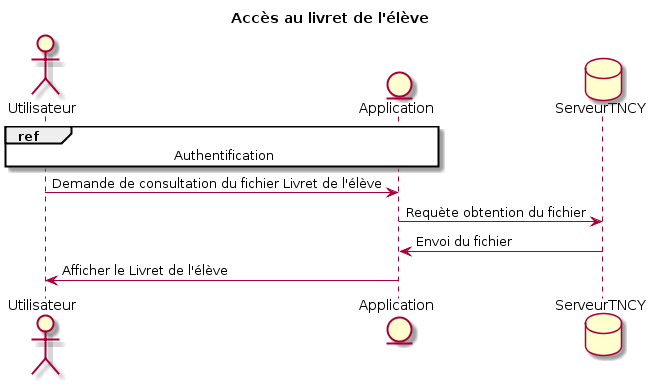
\includegraphics[scale=0.55]{image/accesLivretEleve.png}
\end{center}
\hspace{1cm}Les étudiants doivent pouvoir télécharger le livret de l'élève depuis l'application ; pour ce faire, ils doivent d'abord se connecter au service.

%SAISIE DES INFORMATIONS RELATIVES AU STAGE :
\begin{center}
	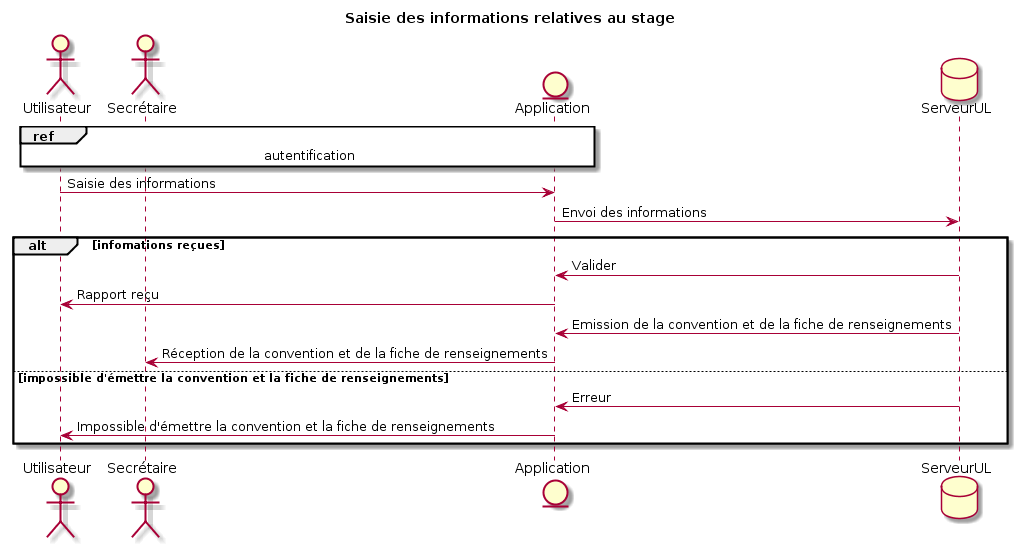
\includegraphics[scale=0.4]{image/saisieInfosStage.png}
\end{center}
\hspace{1cm}Plutôt que de remplir la fiche d'informations relatives au stage et la convention qui doivent ensuite être recopiées manuellement par le secrétarie des stages, l'étudiant a la possibilité d'entrer directement ces informations dans l'application qui émet ensuite automatiquement la convention à signer.

%DEPOSE DU RAPPORT :
\begin{center}
	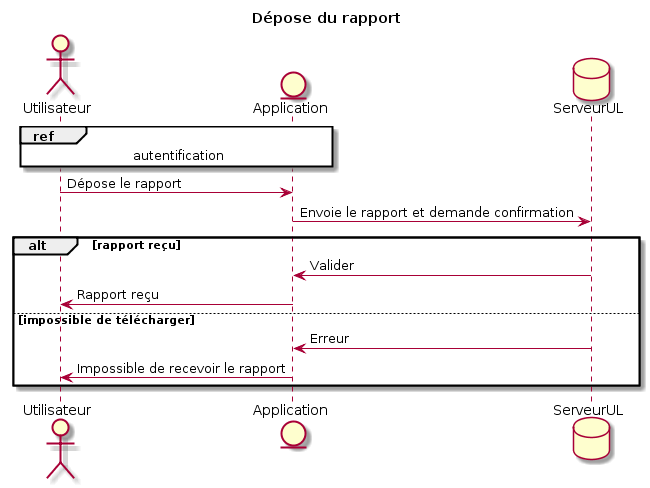
\includegraphics[scale=0.55]{image/deposeRapport.png}
\end{center}
\hspace{1cm}L'une des fonctionnalités principales de l'application est de permettre à l'étudiant de déposer son rapport de stage pour que celui-ci soit corrigé. L'application lui indique si la réception du document a eu lieu ou pas.

%OBTENTION DES DATES DE SOUTENANCE :
\begin{center}
	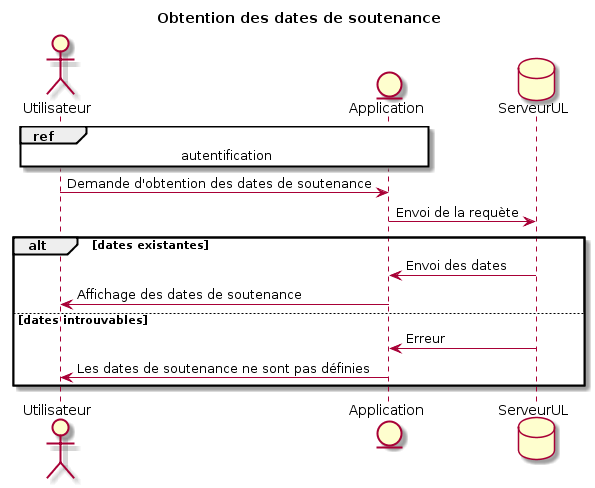
\includegraphics[scale=0.55]{image/obtentionDatesSoutenance.png}
\end{center}
\hspace{1cm}Les étudiants peuvent obtenir les dates de soutenance qui leur sont affectées par l'intermédiaire de l'application après authentification.

%TELECHARGEMENT DE LA FICHE D'EVALUATION :
\begin{center}
	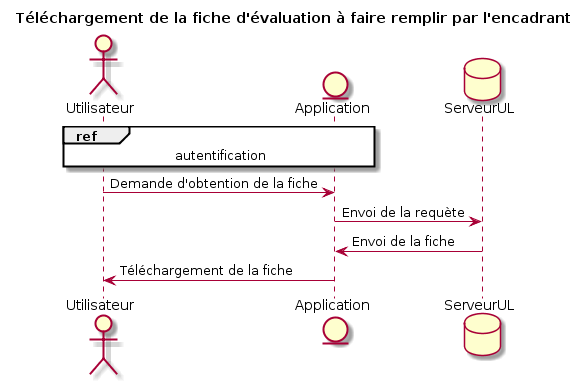
\includegraphics[scale=0.55]{image/telechargementFicheEvaluation.png}
	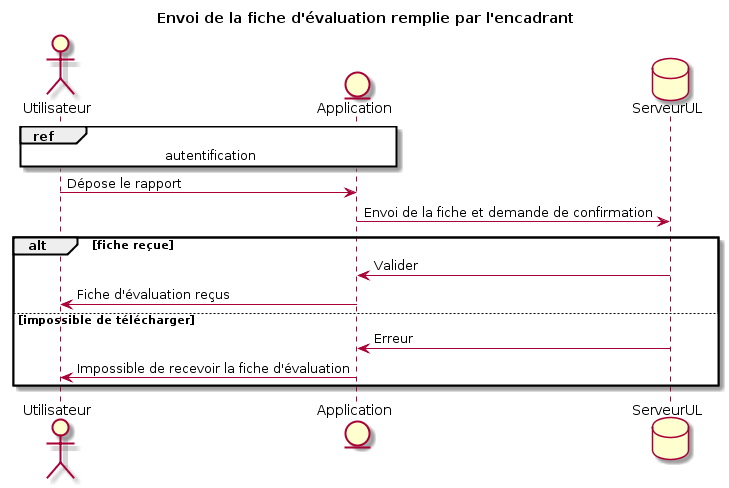
\includegraphics[scale=0.55]{image/envoiFicheEvaluation.png}
\end{center}
\hspace{1cm}L'application permet aux étudiant de télécharger la fiche d'évaluation par le maître de stage pour la lui faire remplir. Après cette opération, ils ont la possibilité de déposer la fiche remplie sur la plateforme.

%MISE EN LIGNE DE DOCUMENTS PAR LE SECRETARIAT DES STAGES :
\begin{center}
	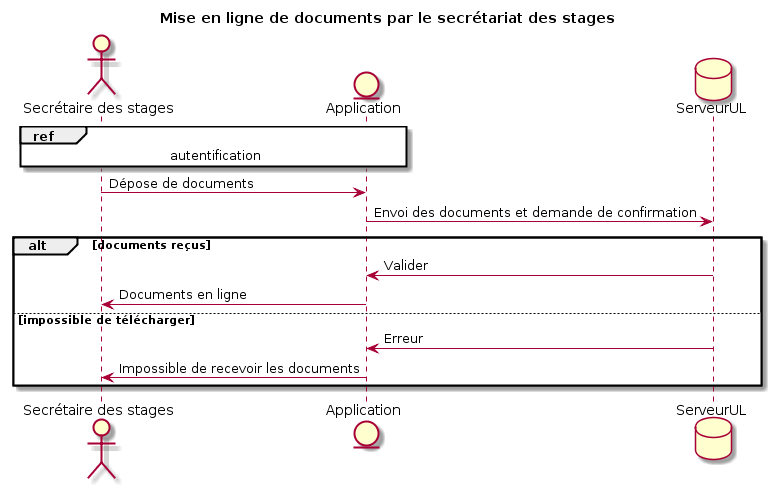
\includegraphics[scale=0.55]{image/miseEnLigneDocumentsParSecretaire.png}
\end{center}
\hspace{1cm}Pour que les étudiants puissent télécharger les documents dont ils ont besoin pour le bon déroulement de leur stage, le secrétariat des stages doit pouvoir les mettre en ligne, accessibles par le biais de l'application développée ici.

%ACCES AUX DONNEES MISES EN LIGNE PAR LES ETUDIANTS PAR LE SECRETARIAT DES STAGES :
\begin{center}
	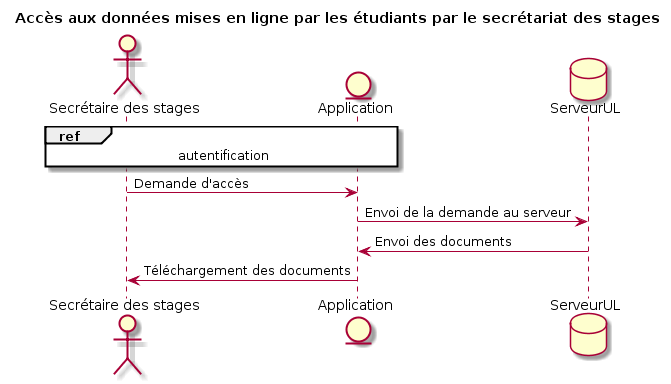
\includegraphics[scale=0.55]{image/accesDonneesParSecretaire.png}
\end{center}
\hspace{1cm}Après que les étudiants ont entré les informations relatives au stage dans l'application, le secrétariat des stages y a accès ainsi qu'a la convention générée automatiquement.

%MODIFICATION DE L'ANNEE D'APPARTENANCE D'UN ETUDIANT PAR LE SECRETARIAT DES STAGES :
\begin{center}
	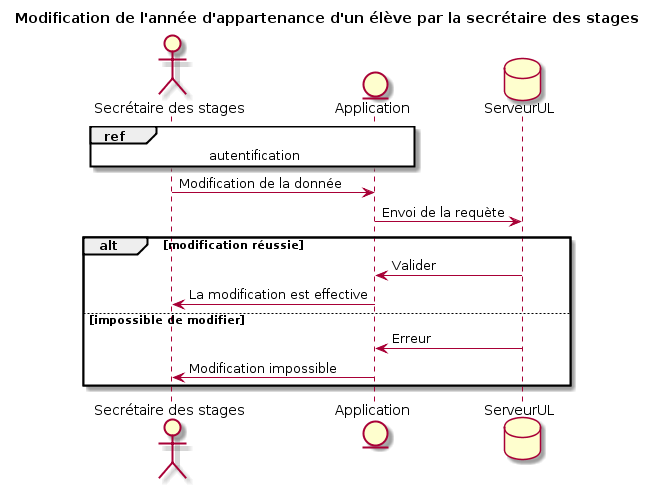
\includegraphics[scale=0.55]{image/modifAnneeParSecretaire.png}
\end{center}
\hspace{1cm}Le secrétariat des stages a la charge de modifier l'année d'appartenance d'un étudiant lorsque son stage est validé par le professeur référent.

%ACCES AUX DONNEES MISES EN LIGNE PAR LES ETUDIANTS PAR LE PROFESSEUR RESPONSABLE :
\begin{center}
	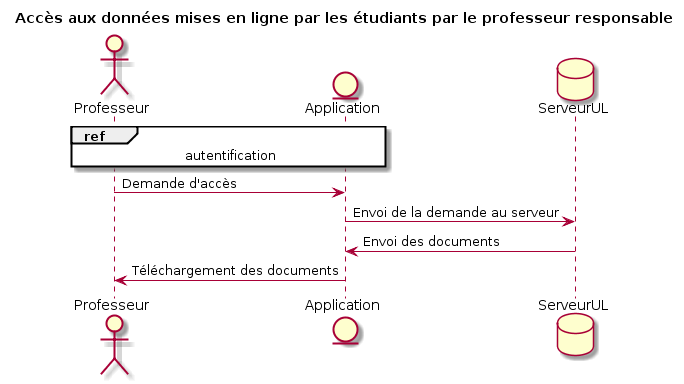
\includegraphics[scale=0.55]{image/accesDonneesParProfesseur.png}
\end{center}
\hspace{1cm}Comme pour le secrétariat des stages, après que les étudiants ont entré les informations relatives au stage dans l'application, leur professeur répérent y a accès.

%VALIDATION OU NON DU STAGE PAR LE PROFESSEUR :
\begin{center}
	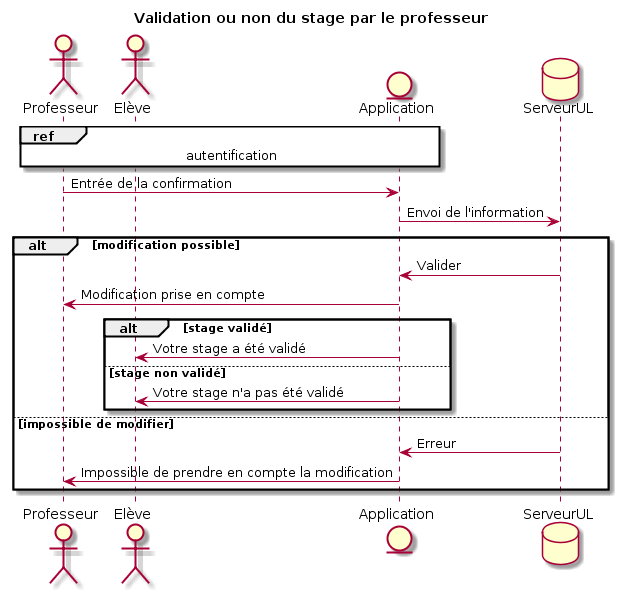
\includegraphics[scale=0.55]{image/validationStage.png}
\end{center}
\hspace{1cm}Après qu'il a corrigé le rapport de stage de l'étudiant et qu'il a consulté la fiche d'évaluation du stage par l'encadrant, le professeur référent a la possibilité de valider ou non le stage de l'élève.

\subsection{Diagrammes de cas d'utilisation}
%DIAGRAMME DE CAS D'UTILISATION DE L'ETUDIANT :
\subsubsection{Diagrammes de cas d'utilisation de l'étudiant}
\begin{center}
	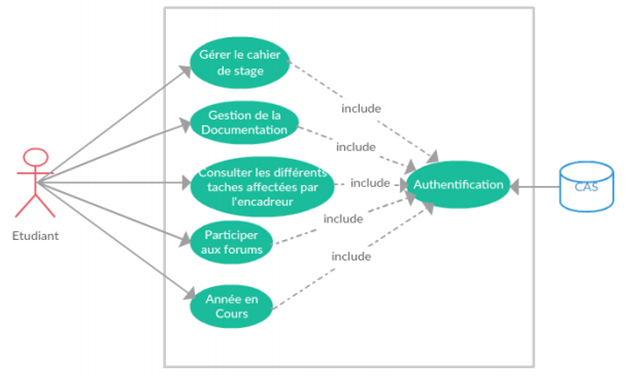
\includegraphics[scale=0.55]{image/casutilisationetudiant.png}
\end{center}
%DESCRIPTION DE CAS D'UTILISATION ANNEE EN COURS :
\subsubsection{Description de cas d'utilisation de l'année en cours}
\begin{center}
	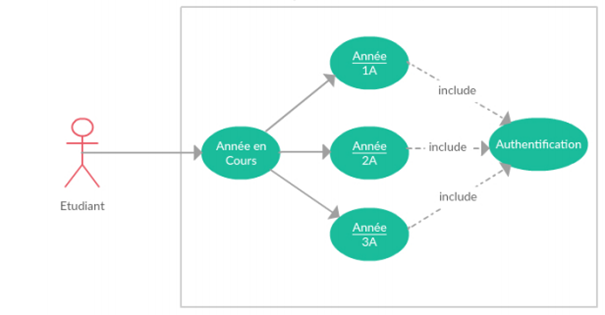
\includegraphics[scale=0.55]{image/descriptiondecasanneencours.png}
\end{center}
%DIAGRAMME DE CAS D'UTILISATION DE L'ENCADREUR :
\subsubsection{Diagrammes de cas d'utilisation de l'encadreur}
\begin{center}
	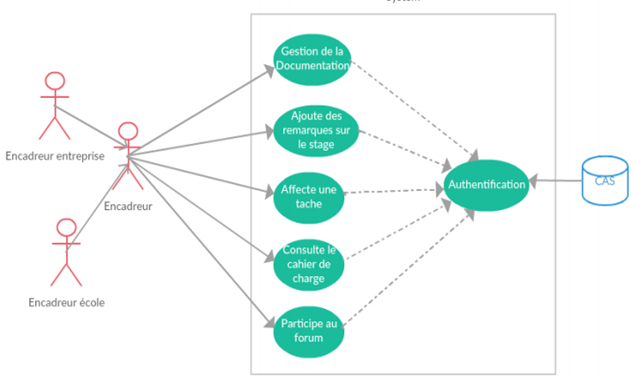
\includegraphics[scale=0.55]{image/casutilisationencadreur.png}
\end{center}
%DIAGRAMME DE CAS D'UTILISATION DU DIRECTEUR :
\subsubsection{Diagrammes de cas d'utilisation du directeur}
\begin{center}
	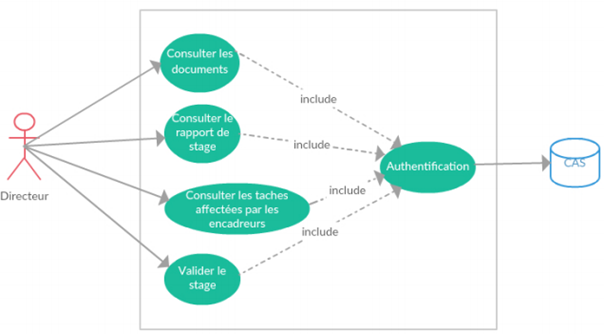
\includegraphics[scale=0.55]{image/casutilisationdudirecteur.png}
\end{center}
%DIAGRAMME DE CAS D'UTILISATION DE L'ADMINISTRATEUR :
\subsubsection{Diagrammes de cas d'utilisation de l'administrateur}
\begin{center}
	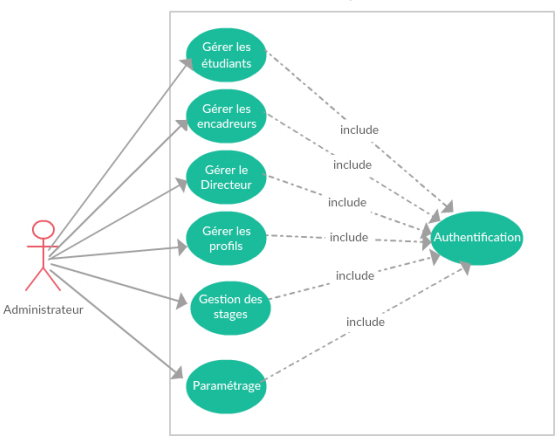
\includegraphics[scale=0.55]{image/casutilisationdeadministrateur.png}
\end{center}


\chapter{AUTRES BESOINS NON FONCTIONNELS}
$<$This template illustrates organizing the functional requirements for the 
product by system features, the major services provided by the product. You may 
prefer to organize this section by use case, mode of operation, user class, 
object class, functional hierarchy, or combinations of these, whatever makes the 
most logical sense for your product.$>$

\section{Besoins liés à la performance}
$<$Dont really say System Feature 1 State the feature name in just a few 
words.$>$

\subsection{Besoins liés à la sécurité}
$<$Provide a short description of the feature and indicate whether it is of 
High, Medium, or Low priority. You could also include specific priority 
component ratings, such as benefit, penalty, cost, and risk (each rated on a 
relative scale from a low of 1 to a high of 9).$>$

\subsection{Besoins liés à la qualité du produit }
$<$List the sequences of user actions and system responses that stimulate the 
behavior defined for this feature. These will correspond to the dialog elements 
associated with use cases.$>$





\chapter{AUTRES BESOINS}



\
\section{ANNEXE A: Dictionnaire de données}

\begin{center}
	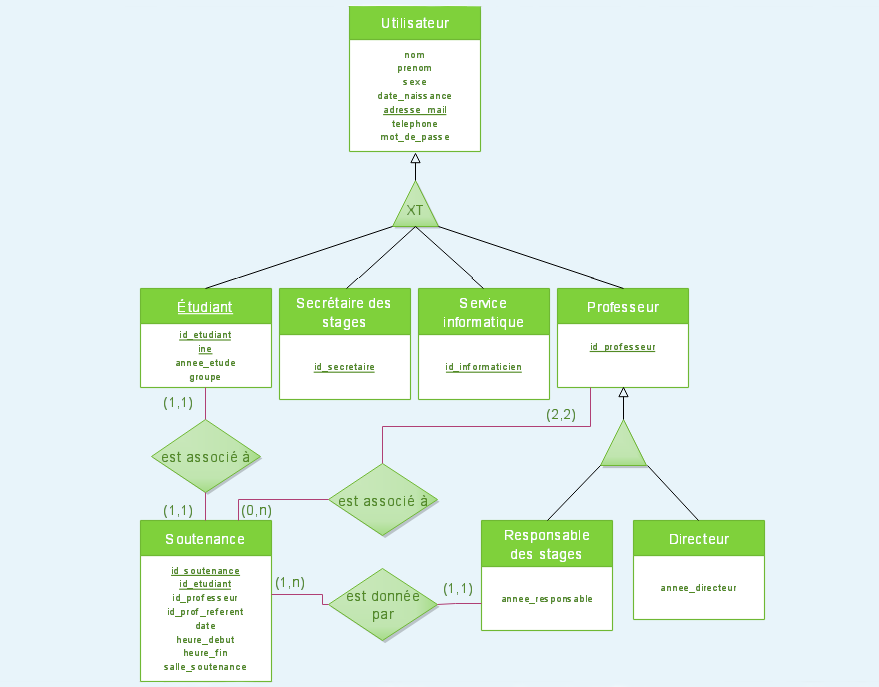
\includegraphics[scale=0.45]{image/diagentiassoc.png}
	\textbf{Figure 5.1.1.} Diagramme entités-associations
\end{center}


\begin{center}
\bf
Étudiants
\end{center}
\begin{tabular}{|l|c|r|}
  \hline
 \bf
 Champ  & Type & Description \\
  \hline
  1.1 & 1.2 & 1.3 \\
  2.1 & 2.2 & 2.3 \\
  \hline
\end{tabular}

\end{document}
